\documentclass[11pt,a4paper,oneside]{book} %scrbook book report
\usepackage{fancyvrb}
\usepackage[
backend=biber,
style=numeric,
sorting=ynt
]{biblatex}
\addbibresource{references.bib}

% Essential packages
\usepackage{amsmath, amssymb, amsthm} % AMS Packages
\usepackage{graphicx,color}           % Packages for graphics and color
\usepackage[left=1.5in, right=1in, top=1in, bottom=1in, includefoot, headheight=13.6pt]{geometry}
\PassOptionsToPackage{printonlyused,smaller}{acronym}
\usepackage{acronym}
% Optional customization packages
\usepackage{lmodern}                  % Custom fonts
\usepackage[T1]{fontenc}              % Ensure correct font encoding
\usepackage{mathptmx}              % Times New Roman Font accross the document

\usepackageamsmath
\usepackage{url}
\usepackage{float}

% Customising chapter headings - sectsty.pdf
\usepackage{sectsty}
\chapterfont{\Large\sc\centering}
\chaptertitlefont{\centering}
\subsubsectionfont{\centering}

\usepackage[hang, small, bf, margin=0pt, tableposition=bottom]{caption}
\setlength{\abovecaptionskip}{10pt}   % Custom captions

% Tables
\usepackage[table]{xcolor}
\usepackage{colortbl}
\usepackage{subfig}

\newcommand{\mc}[2]{\multicolumn{#1}{c}{#2}}
\definecolor{Gray}{gray}{0.83}

\newcolumntype{x}{>{\columncolor{Gray}}c}
\newcolumntype{y}{>{\columncolor{white}}c}

% Page layout
\parindent 0pt
\parskip 1ex
\renewcommand{\baselinestretch}{1.49}
\numberwithin{equation}{section}
\renewcommand{\bibname}{References}
\renewcommand{\contentsname}{Contents}
\pagenumbering{roman}


\newcommand{\acrolabel}[1]{\makebox[3cm][l]{\textbf{#1}}}
\newenvironment{acronyms}{\begin{list}{}{\renewcommand{\makelabel}{\acrolabel}}}{\end{list}}

% \includeonly{tex/chapter1}          % Option to generate specific chapters

% Customising headers - fancyhdr.pdf
\usepackage{fancyhdr}
\pagestyle{fancy}
\rhead{}
\lhead{\nouppercase{\textsc{\leftmark}}}
\renewcommand{\headrulewidth}{0pt}
\makeatletter
\renewcommand{\chaptermark}[1]{\markboth{\textsc{\@chapapp}\ \thechapter:\ #1}{}}
\makeatother


% Hyperreferencing and citations
\usepackage{hyperref}
\hypersetup{
    colorlinks,
    citecolor=black,
    filecolor=black,
    linkcolor=black,
    urlcolor=black
}

% Section symbol
\usepackage{cleveref}
\crefname{section}{\S}{\S\S}
\Crefname{section}{\S}{\S\S}
\crefname{subsection}{\S}{\S\S}
\Crefname{subsection}{\S}{\S\S}


\usepackage{tabu}
\usepackage{adjustbox}
\usepackage{booktabs}% for better rules in the table
\usepackage{graphicx}
%\usepackage{subfigure}
%\usepackage{color}
%\usepackage{colortbl}
%\usepackage{soul}
%\usepackage{listings}
%\lstloadlanguages{Java,XML}
%\lstset{frame=lines}
\usepackage{./styles/astron}
%\usepackage{xspace}
%\usepackage[leqno]{amsmath}
%\usepackage{hyperref}
%\usepackage{sfmath}
%\usepackage{setspace} 
\usepackage{./styles/nust}
\graphicspath{{./img/}{./figs/}}

\title{Enhancing Cybersecurity: AI Strategies for Phishing Detection and Prevention}
%\subtitle{A sub-title}

\author{
  Matteo Giorgi
}
\degree{Artificial Intelligence and Data Engineering DII \\ ICT Risk Assessment} % MSCSE, MSCCS %% Degree Title and It's abbreviation
\school{University of Pisa } %SChool abbreviation and Full Name
%\adviser{Supervisor Name}
%\adviserAffiliation{Department of Information Engineering}

\date{September 2024}

% \setcounter{tocdepth}{2}
% \setstretch{1.1}
% \linespread{1.1}
\usepackage{listings}
\usepackage{svg}
\usepackage{graphicx}

% Impostazioni di base per il pacchetto listings
\lstset{
    basicstyle=\ttfamily,
    breaklines=true,
    showstringspaces=false,
    language=C,
    commentstyle=\color{green!50!black},
    keywordstyle=\color{blue},
    numberstyle=\tiny\color{gray},
    numbers=left,
    frame=single
}

\begin{document}
\maketitle
\tableofcontents
\listoffigures
\newpage
\input{preface/Abstract}

\resetpagenumbering

\chapter{Introduction}
In recent years, the widespread use of the internet for activities such as communication, online shopping, and various other online services has led to a significant increase in the amount of personal information circulating online. This surge has, in turn, exposed users to various cyber threats, with phishing being one of the most common. According to a 2017 FBI report, 25,344 phishing scams were identified, resulting in a total loss of \$29,703,421, primarily impacting sectors like finance, email, cloud storage and hosting, e-commerce, telecommunications, and social media. These numbers have been rising each year; in fact, a 2021 report from the Anti-Phishing Working Group identified 611,877 phishing sites, nearly six times the number identified in 2020. It is therefore crucial to find a solution to this type of cyber threat.

\section{The phishing threat}
Phishing is a type of cybercrime and social engineering attack designed to obtain sensitive information such as login credentials and financial details. These attacks often exploit human emotions, such as fear, urgency, or curiosity, to manipulate victims into divulging their confidential information. Attackers commonly utilize social media platforms, emails, and other forms of online communication to deceive their targets, directing them to fraudulent websites that appear legitimate.

There are various types of phishing attacks that can be categorized based on the target, the medium used, and the method employed. In this document, we will focus on social engineering attacks that occur through the creation of fake websites. These fake websites are shared with victims via links embedded in advertisements, within cracks of licensed software, or in phishing emails.

Phishing attacks are now more robust and hard to detect because the attacker uses various techniques, such as \textbf{Browsers in the Browser attacks} (BiTB) attacks, \textbf{Watering Hole} Attacks or \textbf{Clickjacking} to bypass the current detection systems as presented in the document of \textcite{PhishTransformer}

BiTB Attacks involve a malicious website running within a legitimate one by exploiting browser vulnerabilities. This is achieved through hidden iframes or windows that deceive users into interacting with malicious content unknowingly, such as clicking on links or entering personal information.

Watering Hole Attacks compromise legitimate websites frequented by targeted users. Attackers insert malicious links that redirect users to fraudulent webpages when clicked, tricking users into divulging sensitive information or inadvertently installing malware.

Clickjacking employs transparent overlays or hidden links to deceive users into clicking unintended buttons or links on webpages. Users unknowingly perform actions on malicious sites, such as installing malware or disclosing confidential information.

These attacks represent sophisticated strategies that exploit both user behavior and technical vulnerabilities in web environments. Unlike traditional attacks such as Cross-Site Scripting (XSS), Session Hijacking, or Malware Phishing, which exploit specific code or protocol weaknesses, BiTB, Watering Hole, and Clickjacking focus on manipulating user-content interactions to gain unauthorized access or steal sensitive data.

Understanding these mechanisms is essential for implementing effective security measures and safeguarding users and digital infrastructures against evolving cyber threats.

\section{Existing approaches}
There are several methods to recognize and block phishing attacks, which can be broadly classified into two main categories: \textbf{Content-Based} and \textbf{Non-Content-Based} techniques.

\subsection*{Non-Content-Based Techniques}
These methods focus on features other than the website's content. Examples include:
\begin{itemize}
    \item \textbf{Blacklisting and Whitelisting}: This involves maintaining an updated list of URLs marked as either malicious or safe. Continuous updates are necessary for this method to remain effective.
    \item \textbf{DNS Analysis}: This technique verifies the authenticity of a domain by analyzing its DNS information.
\end{itemize}

\subsection*{Content-Based Techniques}
Content-based approaches are particularly interesting because they analyze the actual content of a website to detect phishing attacks. Some of the key approaches in this category include:
\begin{itemize}
    \item \textbf{URL Analysis and Visual Similarity}: This involves examining the characteristics of a URL, such as the presence of IP addresses, URL length, and special characters, to determine whether a site is legitimate. This approach is often combined with content analysis, which identifies visual similarities with popular legitimate sites, for instance, by comparing CSS rules or performing image and text analysis.
    \item \textbf{Spam Filters}: These techniques address the phishing problem at an earlier stage by detecting and filtering fraudulent emails, thus preventing users from falling into phishing traps in the first place.
\end{itemize}

\subsection*{Advanced Techniques Using Artificial Intelligence (AI)}
More innovative and recent techniques involve the use of AI to detect phishing attempts. Among these, we can distinguish:
\begin{itemize}
    \item \textbf{Machine Learning (ML) Approaches}: These techniques use classification algorithms (such as Support Vector Machines (SVM), Decision Trees (DT), K-Nearest Neighbors (KNN), and Random Forests (RF)) to differentiate between legitimate and fraudulent websites. In these approaches, it's necessary to extract a set of features that best represent a website.
    \item \textbf{Deep Learning (DL) Techniques}: These approaches use neural networks, such as Convolutional Neural Networks (CNN) and Recurrent Neural Networks (RNN), to classify websites. Unlike ML techniques, DL methods automatically extract the most relevant features, making the model more complex and often less interpretable, which is why they are sometimes referred to as "black-box models."
    \item \textbf{Transformers}: Even more recent techniques involve the use of Transformers, such as encoders combined with CNNs, to encode the website's features and discover the relationships between them that enable the classification task.
\end{itemize}

\section{Evaluation Metrics}
In the context of machine learning and classification, there are several common metrics used to evaluate the performance of a model. Among these, \textit{Accuracy}, \textit{Precision}, \textit{Recall}, and \textit{F1-Score} are particularly important.

\subsection*{Accuracy}
Accuracy measures the proportion of correct predictions out of the total number of samples. It is defined as:

\begin{equation}
\text{Accuracy} = \frac{TP + TN}{TP + TN + FP + FN}
\end{equation}

Where:
\begin{itemize}
    \item $TP$ (True Positives) are the correctly predicted positive instances.
    \item $TN$ (True Negatives) are the correctly predicted negative instances.
    \item $FP$ (False Positives) are the incorrectly predicted positive instances.
    \item $FN$ (False Negatives) are the incorrectly predicted negative instances.
\end{itemize}

\subsection*{Precision}
Precision is the proportion of true positives among all instances that were classified as positive. It is calculated as:

\begin{equation}
\text{Precision} = \frac{TP}{TP + FP}
\end{equation}

\subsection*{Recall}
Recall, also known as sensitivity, is the proportion of true positives compared to the total number of actual positive samples. It is calculated as:

\begin{equation}
\text{Recall} = \frac{TP}{TP + FN}
\end{equation}

\subsection*{F1-Score}
The F1-Score is the harmonic mean of precision and recall, and it is particularly useful when you need to balance these two metrics. It is defined as:

\begin{equation}
\text{F1-Score} = 2 \cdot \frac{\text{Precision} \cdot \text{Recall}}{\text{Precision} + \text{Recall}}
\end{equation}
 
\chapter{Literature Review}
In this document, we will analyze three AI-based approaches for classifying websites and preventing phishing. The first approach involves the creation of an anti-phishing browser based on ML \textbf{\textcite{EPDB}}. The second approach utilizes Generative Adversarial Networks (GANs) \textbf{\textcite{PDGAN}}. Finally, the third approach employs a Transformer model for website classification \textbf{\textcite{PhishTransformer}}.

\section{Embedded Phishing Detection Browser}

\subsection{System Overview}
The authors propose a comprehensive solution by introducing a new browser equipped with an intelligent unit capable of analyzing web pages and detecting phishing attempts. Specifically, the system comprises several key components: a \textbf{user interface}, which allows the user to interact with the browser and includes features such as the address bar, navigation buttons, and more; a \textbf{browser engine}, responsible for loading websites and enabling navigation; a \textbf{rendering engine}, tasked with converting the URL into a graphical format by interpreting HTML, XML, CSS, and other elements; and \textbf{additional submodules} for interpreting JavaScript, communicating via networking protocols, and managing data storage. These components are fundamental and present in any browser.

To enhance phishing detection and prevention, the authors also integrate an \textbf{intelligent engine} that analyzes web pages and alerts the user to potential threats. This module operates in parallel with the browser engine, ensuring that it does not impact the browser's performance. The diagram in the figure illustrates the mentioned components and their interdependencies.

\begin{figure}[htp]
    \centering
    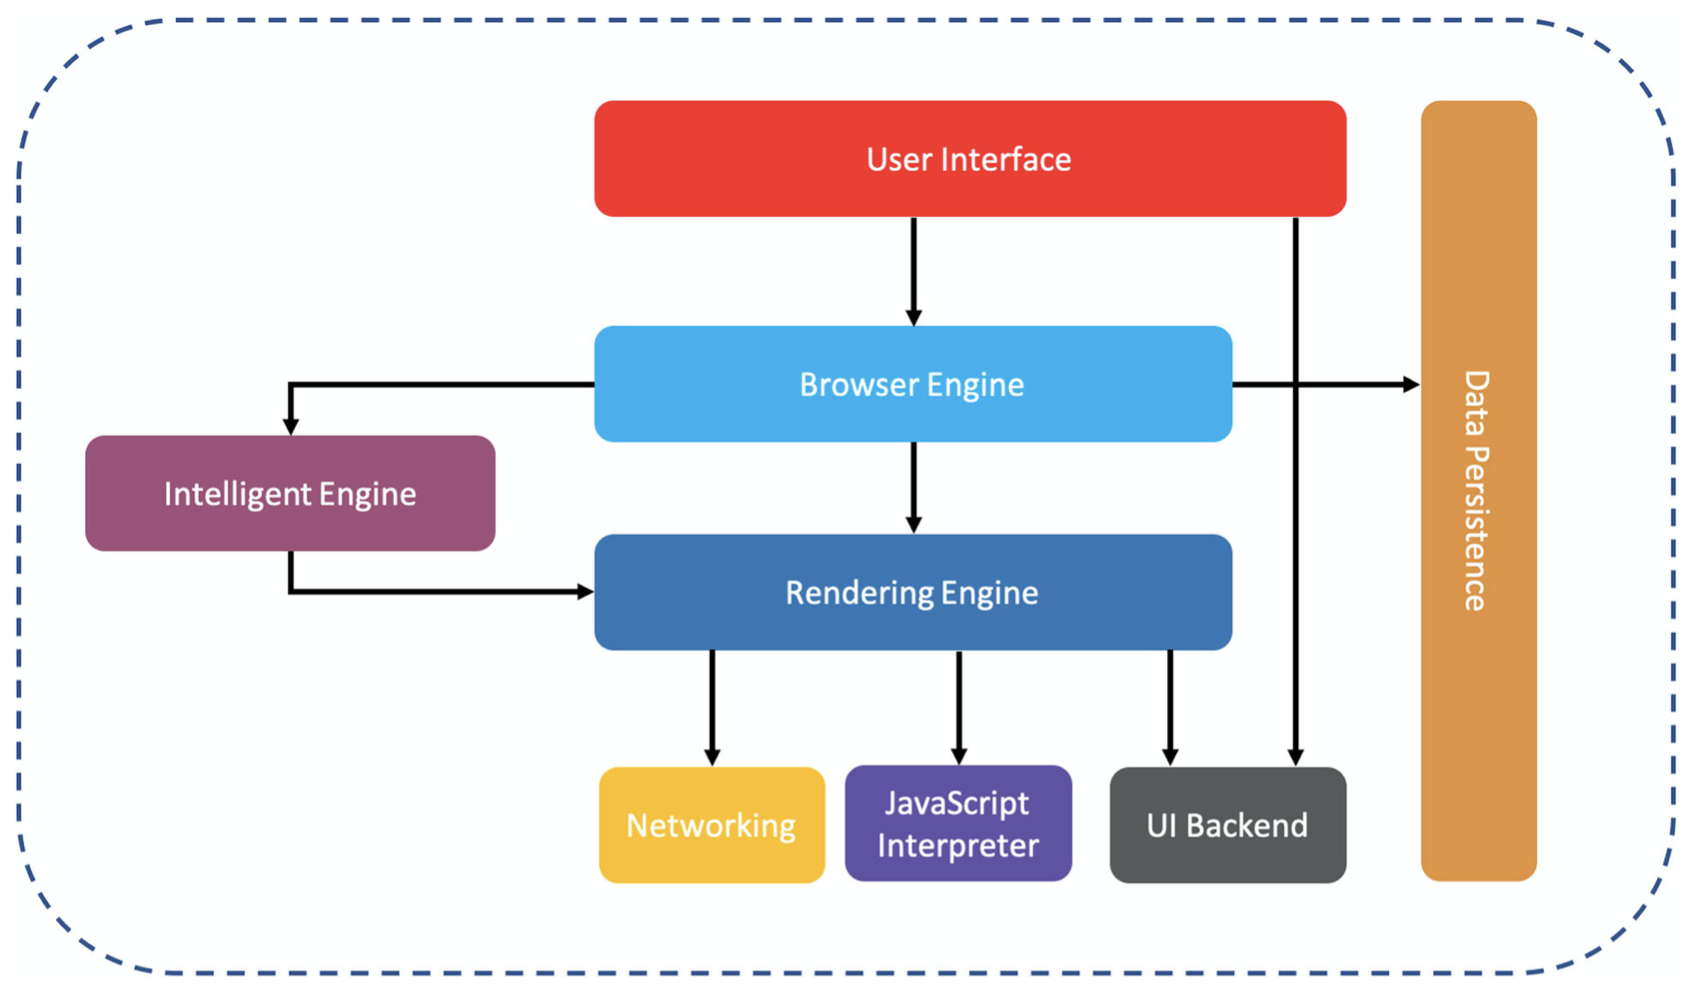
\includegraphics[width=0.8\linewidth]{images/EPDB_scheme.png}
    \caption{EPDB scheme}
    \label{fig:EPDB scheme}
\end{figure}

The system extracts 30 features from the URL, which are used by the intelligent module to detect a fraudulent site. If a phishing site is detected, the user is notified through a popup, allowing them to either stop or continue browsing. In the case of a phishing site, the execution of JavaScript code is halted, which is not something current browsers typically do. The ML model is stored in a pickle file and can be easily updated and redistributed.

\subsection{Dataset and Model}
To create the intelligent system, data from PhishTank and MillerSmiles were used. The dataset includes 11,055 records, with each record consisting of 30 features associated with the URL, allowing for the differentiation between fraudulent and safe websites.

The ML model employed to build the intelligent system is the Random Forest, an ensemble model of decision trees. Decision trees are easily interpretable, making it straightforward to understand which characteristics of a URL lead to its classification. However, these models are prone to overfitting, meaning they may adapt too closely to the training data and struggle to generalize effectively. To address this issue and achieve optimal performance, the authors used GridSearchCV to find the best model hyperparameters.

For training, the K-fold cross-validation technique was used. This involves performing K, in this case K=5, iterations where the dataset is divided into partitions (training and test), and the model is trained on these. The process is repeated K times, and an average of the model's performance is obtained.

It is interesting to see which features contributed the most to identifying fraudulent sites versus safe ones. The following graph highlights the most significant features in the case of the Random Forest model.

\begin{figure}[htp]
    \centering
    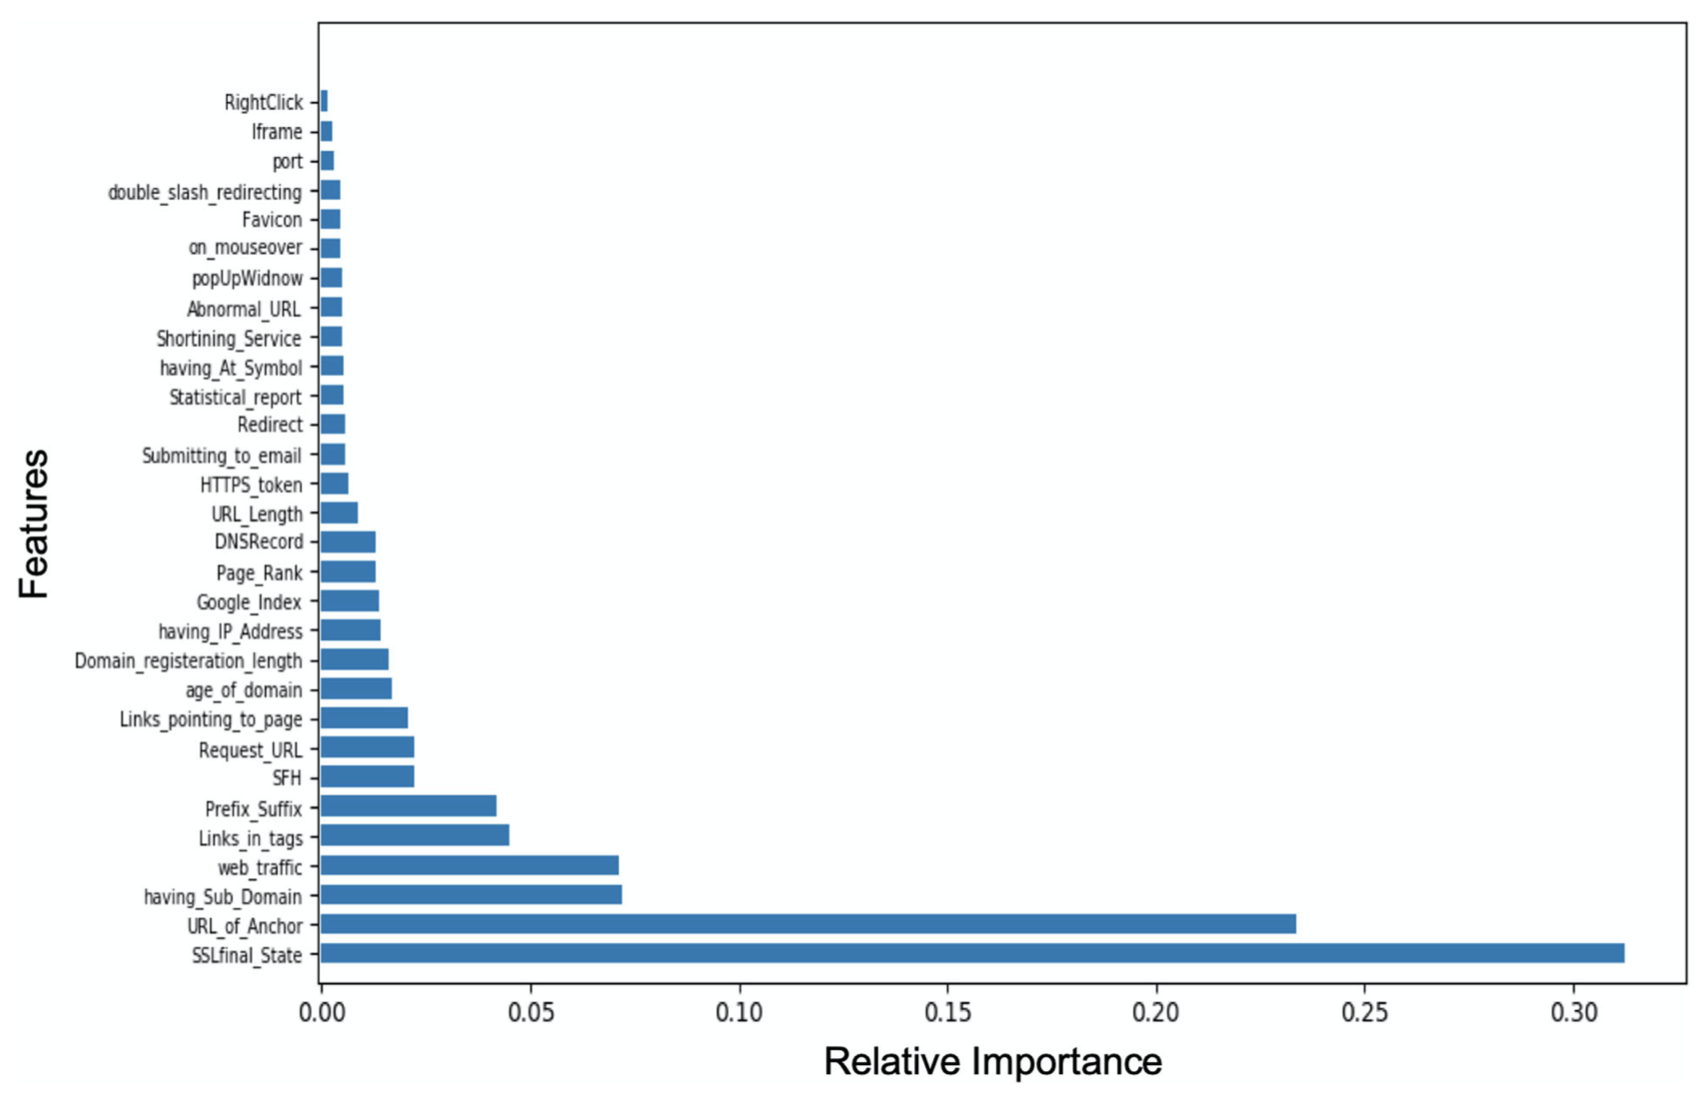
\includegraphics[width=1\linewidth]{images/30features_importance.png}
    \caption{Model-Based feature importance of 30 features}
    \label{fig:Relative importance of features}
\end{figure}
The 5 most important features are as follows:

\begin{enumerate}
    \item \textbf{SSLfinal\_State}: 
         This feature refers to the state of the site's SSL/TLS certificate. A valid and up-to-date SSL certificate is a signal of authenticity and security. In contrast, the lack of a certificate or the presence of an expired certificate could indicate a malicious site. 
         It is the most important feature because many phishing sites do not invest in proper SSL certificates or use short-lived certificates to avoid detection.
    
    \item \textbf{URL\_of\_Anchor}:
         This feature considers the percentage of links within the page that point to external domains compared to those that point to the same domain. A high number of outbound links can be indicative of phishing, as legitimate sites tend to have consistent internal links.
    
    \item \textbf{having\_Sub\_Domain}:
        This feature evaluates the presence and number of subdomains in the URL. A high number of subdomains or the use of unusual subdomains can be an indicator of a phishing site.
        Phishing attacks often use subdomains to mask suspicious URLs, making the URL appear similar to that of a legitimate site.
    
    \item \textbf{web\_traffic}:
        This feature analyzes the website's traffic using webpage rank. Sites with low traffic can be suspicious, as a legitimate site tends to have consistent and significant traffic.
        A phishing site usually has low web traffic since it is not regularly visited by normal users, but only by the victims of the attack.
    
    \item \textbf{Links\_in\_tags}:
        This feature measures the percentage of links within HTML tags (such as \texttt{<a>}, \texttt{<script>}, \texttt{<link>}, etc.). Phishers might insert malicious links into these tags to redirect users to phishing sites.
        A high percentage of links within these tags can be a direct indicator of a phishing attempt.
\end{enumerate}

The chart clearly shows that not all features contribute equally to the classification of a URL as benign or malicious. Some features, such as \textbf{RightClick} or \textbf{iframe}, have very low relative importance, indicating they are not strong indicators of phishing. In contrast, \textbf{SSLfinal\_State} and \textbf{URL\_of\_Anchor} are among the most important features, suggesting that the presence of a valid SSL certificate and the structure of the links within the site are key factors in determining the legitimacy of a site.

\subsection{Models Evaluations}
To determine the most suitable ML model for this task, SVM and Logistic Regression were also trained. The best model turned out to be the Random Forest, with an accuracy of 99.36\% and an F1-score of 99.43\%. The figure shows the confusion matrices for the three models mentioned.

\begin{figure}[htp]
    \centering
    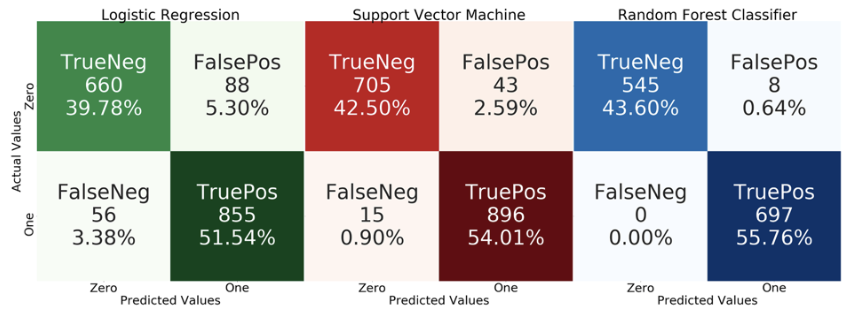
\includegraphics[width=1\linewidth]{images/ML_comparison.png}
    \caption{Confusion Matrix of ML models}
    \label{fig:Confusion Matrix of ML models}
\end{figure}

Another experiment focused on performance in terms of execution time. On average, the EPDB model was able to analyze a site in 4 seconds compared to 6 seconds for the Chrome extension, making this client-side solution more efficient.

\section{Phishing Detection with Generative Adversarial Network}

\subsection{System Overview}
The authors of this solution also adopted a completely URL-based approach, without considering the page content or third-party services. The system is structured as a \textbf{GAN}, which involves two Artificial Neural Networks (ANN) trained in an adversarial manner. Specifically, there is a generator, composed of a Long Short-Term Memory (LSTM) network, responsible for generating synthetic URLs (both fraudulent and legitimate). The discriminator, on the other hand, is a CNN tasked with analyzing the URL and classifying it as either legitimate or phishing.

The generator is trained to maximize the error made by the discriminator in recognizing the URL as synthetic, which indicates that it is improving in generating artificial URLs. Meanwhile, the discriminator is trained to recognize the generated URLs as accurately as possible, hence the term "adversarial neural networks."

Below is the structure proposed by the authors.

\begin{figure}[htp]
    \centering
    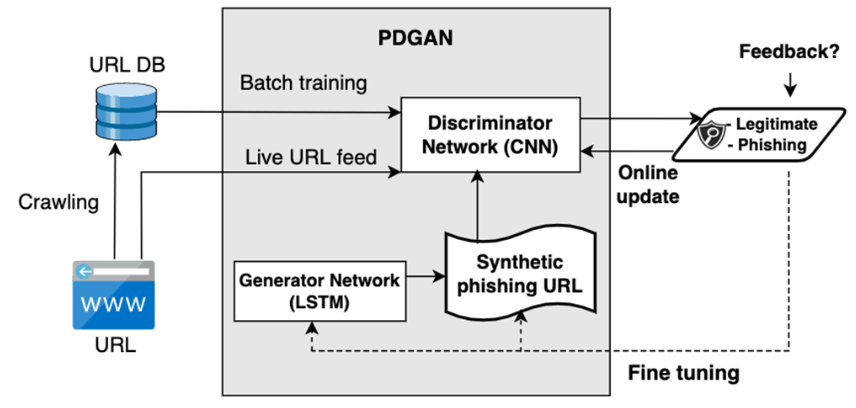
\includegraphics[width=0.8\linewidth]{images/PDGAN system.png}
    \caption{PDGAN Workflow}
    \label{fig:PDGAN Workflow}
\end{figure}

\subsection{Dataset and Model}
In this case as well, the dataset used comes from PhishTank, specifically MUPD, a balanced collection of 4.5 million URLs. After preprocessing (removing duplicates and balancing), the dataset is reduced to 2.3 million URLs. The preprocessed dataset is then randomly split into 60\% training, 20\% validation, and 20\% test sets. Since it is a balanced dataset, accuracy can be used as a metric to evaluate performance.

URLs cannot be directly fed into the model as plain text, so further preprocessing of the dataset is required to train the model. Specifically, it is assumed that the URL length does not exceed 255 characters, in accordance with the RFC2616 protocol. If it exceeds this limit, the URL is truncated; if it is shorter, zero padding is applied. Considering an alphabet of 69 characters (letters, numbers, and special characters), a one-hot vector is generated for each character in the URL, with a value of 1 corresponding to the represented character and all other characters set to 0, as shown in the figure.

\begin{figure}[htp]
    \centering
    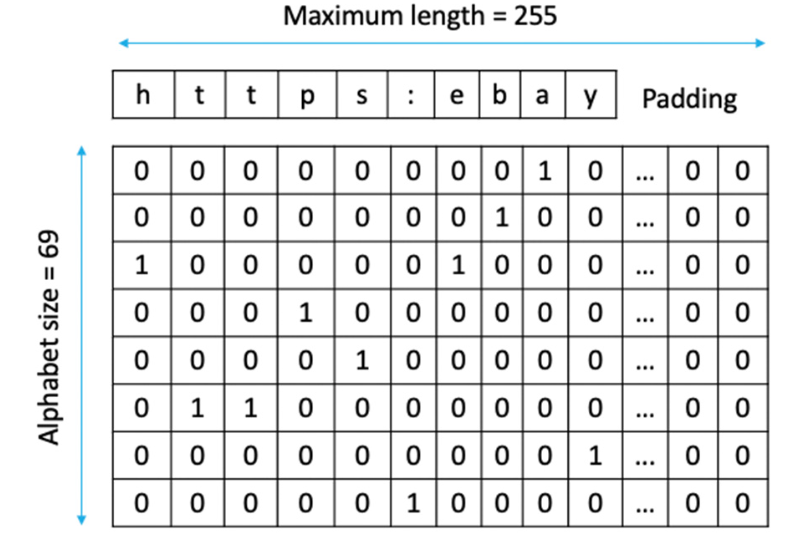
\includegraphics[width=0.8\linewidth]{images/URLs_preprocessing.png}
    \caption{URLs encording}
    \label{fig:URLs encording}
\end{figure}

This process is repeated for all URLs, and at this point, the dataset is ready to be used in the GAN.

\subsubsection{Generator}
The generator, as previously mentioned, is an LSTM, a type of network well-suited for storing long sequences of information. The structure of these networks consists of a set of memory cells connected to each other. Each cell has three main gates: the forget gate, the input gate, and the output gate. These gates regulate the flow of information into and out of the cell, enabling the LSTM to maintain and update its internal state over time.

\begin{figure}[htp]
    \centering
    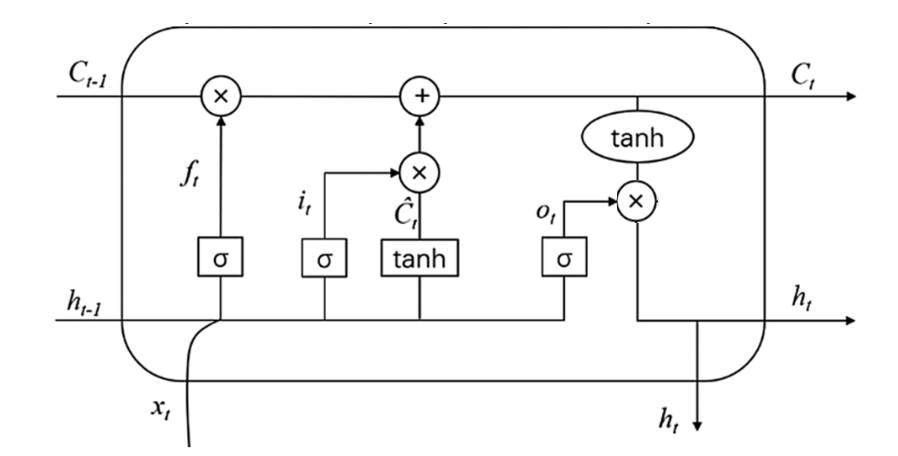
\includegraphics[width=0.8\linewidth]{images/generator_structure1.png}
    \caption{LSTM Cell}
    \label{fig:LSTM Cell}
\end{figure}

\textbf{Forget Gate}: The forget gate decides what information from the previous cell state \(C_{t-1}\) should be discarded. It outputs a value between 0 and 1 for each number in the cell state \(C_{t-1}\), where 1 represents "completely keep this" and 0 represents "completely forget this."
\[f_t = \sigma(W_f*[h_{t-1},x_t] + b_f)\]

\textbf{Input Gate}: The input gate determines which values from the input \(x_t\) will be used to update the cell state. It controls how much of the new input \(x_t\) should be added to the current cell state. 
\[i_t = \sigma(W_i*[h_{t-1},x_t] + b_i)\]

\textbf{Cell State Update}: The cell state \(C_t\) is then updated by combining the previous cell state \(C_{t-1}\) and the new candidate values \(\tilde{C}_t\) (scaled by the forget gate \(f_t\) and the input gate \(i_t\) respectively).
\[
C_t = f_t \otimes C_{t-1} \oplus i_t \otimes \tanh(W_c \cdot [h_{t-1}, x_t] + b_c)
\]

\textbf{Output Gate}: The output gate determines what the next hidden state \(h_t\) should be. This hidden state \(h_t\) is also used as the output of the LSTM cell. The output is based on the current cell state \(C_t\), passed through a \(\tanh\) function, and modulated by the output gate.
\[o_t = \sigma(W_o*[h_{t-1},x_t] + b_o)\]

In these equations, \(x_t\) is the input to the current layer, \(\sigma\) is the sigmoid function, \(h_{t-1}\) represents the hidden state at time \(t-1\), and \(b\) represents the bias for each gate. \(W_f\), \(W_i\), and \(W_o\) are the weight matrices for the connections.

Finally, the output of the LSTM cell, \(h_t\), is computed by combining the output gate \(o_t\) with the updated cell state \(C_t\), scaled through a \(\tanh\) function.
\[
h_t = o_t \otimes \tanh(C_t)
\]

\begin{figure}[htp]
    \centering
    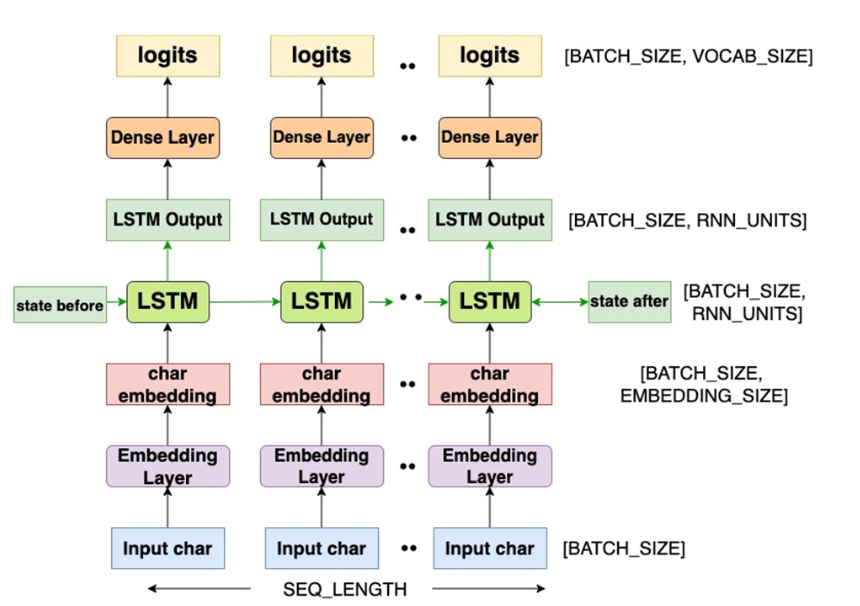
\includegraphics[width=0.8\linewidth]{images/generator_structure2.png}
    \caption{Generator architecture}
    \label{fig:Generator architecture}
\end{figure}

\subsubsection{Discriminator}
The discriminator is a CNN consisting of 9 layers in depth, with 6 convolutional layers and 3 fully connected dense layers. One-dimensional filters were used, which are convolutional filters that move in only one direction. Max-pooling layers were employed to extract the most relevant features and reduce the dimensionality, and dropout layers were used to decrease the number of network parameters, thereby reducing the likelihood of overfitting.

\subsubsection{DPGAN parameters}
For both models, binary cross-entropy was used as the loss function, with a learning rate of \textbf{0.001} and the Adam optimizer. The best results were achieved with \textbf{256} hidden layers and a batch size of \textbf{64} for the generator, at epoch 80. As for the discriminator, training was stopped at the twentieth epoch, and the best results were obtained using a convolutional kernel size of \textbf{{7,7,3,3,3,3}} and a batch size of \textbf{128}.

\subsection{Models Evaluations}
The authors compared their model with other similar models in the literature, specifically deep learning models that are URL-based and use the same dataset. Notably, PUCNN employs a CNN to extract character-level feature representations of URLs, while PDRCNN is based on a two-dimensional URL representation. It uses a biLSTM network to extract the global features of the constructed tensor and a CNN to extract the local features. 

\begin{figure}[htp]
    \centering
    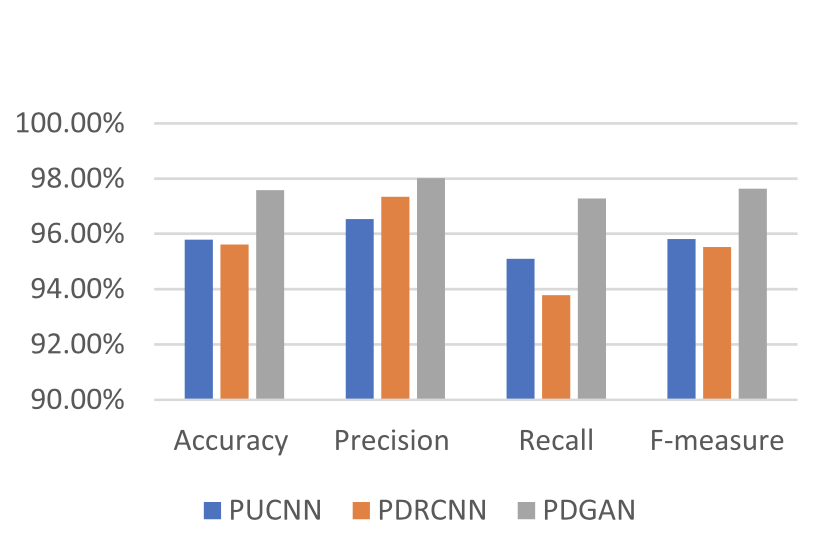
\includegraphics[width=0.8\linewidth]{images/DPGAN comparisongraph.png}
    \caption{DPGAN and Baselines comparison}
    \label{fig:DPGAN and Baselines comparison}
\end{figure}

The graph shows the results, highlighting that the DPGAN model achieved 98.02\% precision and 97.58\% accuracy, benefiting from the data augmentation provided by the generator.

\section{Phishing Detection using Transformer}

\subsection{System Overview}
The authors of this model propose a hybrid approach that combines URL-based analysis with partial content analysis of the web page to prevent the phishing attacks mentioned at the beginning of the document (BITB, Watering Hole, Clickjacking). Specifically, they suggest analyzing the URLs contained within the HTML and JavaScript code of the page in question to avoid the issue of embedding malicious code in legitimate content. This approach, therefore, strikes a balance between a purely URL-based approach (which is very fast but less accurate) and a content-based approach that analyzes the HTML, JavaScript, CSS, and DOM (which is much more accurate but also more complex and slower).

As shown in the figure, the system consists of a scraping and preprocessing phase. The collected data is then passed to a CNN, which extracts local features, followed by a Transformer encoder that encodes and identifies long-range dependencies among the various encodings to accurately classify the URL.

\begin{figure}[htp]
    \centering
    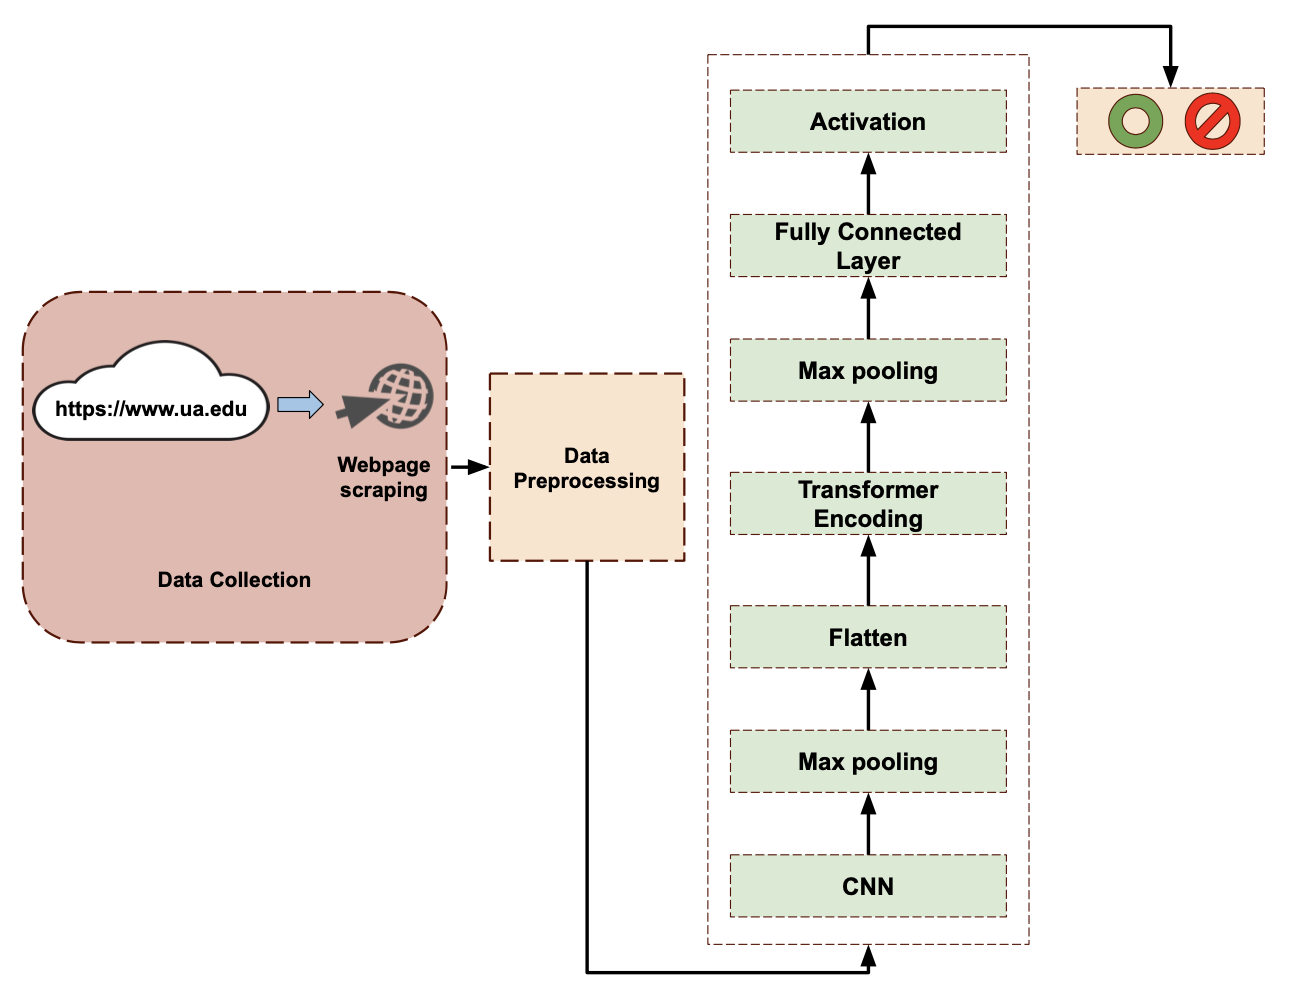
\includegraphics[width=0.8\linewidth]{images/transformer schema.png}
    \caption{CNN+Transformer schema}
    \label{fig:CNN+Transformer schema}
\end{figure}

\subsection{Dataset and Model}
The dataset consists of a collection of 50,000 malicious URLs from Phishtank and PhishArmy and a collection of 50,000 benign URLs from Alexa. For each URL, the online presence of the webpage was verified; if the page was not accessible, the URL was removed. If the page was accessible, web scraping was performed on the URL to retrieve all the URLs within the webpage, creating a list associated with the original URL \(X_i\) in the form \(X_i = [u_1,u_2,...,u_m]\). Thus, the final dataset is a matrix of the type \(D = [X_1,X_2,...,X_n]\).

The balanced dataset was partitioned into 70\% training, 20\% test, and 10\% validation.
\subsubsection{Preprocessing}
The preprocessing phase is quite important and consists of data scraping, cleaning, tokenization, and concatenation. Half of the URLs were found to be offline, so the final dataset consists of 50,000 URLs balanced between the classes. For tokenization, the authors use character-level tokenization, which allows the handling of unknown words. The possible characters considered include 92 options, including letters, numbers, and special characters. Additionally, four indices are introduced: `<PAD>` for padding, `<UNK>` for unknown characters, `<STA>` to mark the start of a URL, and `<SEP>` to mark the end of a URL.

The URL takes the form \(u = [c_1,c_2,...,c_d]\), with \(d\) being the fixed length of the URL. If a URL is longer than \(d\), it is truncated; if it is shorter, padding characters `<PAD>` are added. The same approach is applied to the lists of URLs contained within the target URL. If the list exceeds the limit of URLs per page, the excess URLs are removed; otherwise, padding URLs of the form `[<STA>,<PAD>,...,<PAD>,<SEP>]` are added. 

To determine the maximum URL length and the maximum number of URLs per page, an analysis was conducted on the data by class to choose the appropriate parameters. On average, a benign page is 62 characters long and contains 114 URLs, while a malicious page is 56 characters long and has 11 embedded URLs. The maximum number of characters per URL was set to 100 to allow some margin for error, and the maximum number of embedded URLs was set to 100 to avoid favoring either class.
\begin{figure}[htp]
    \centering
    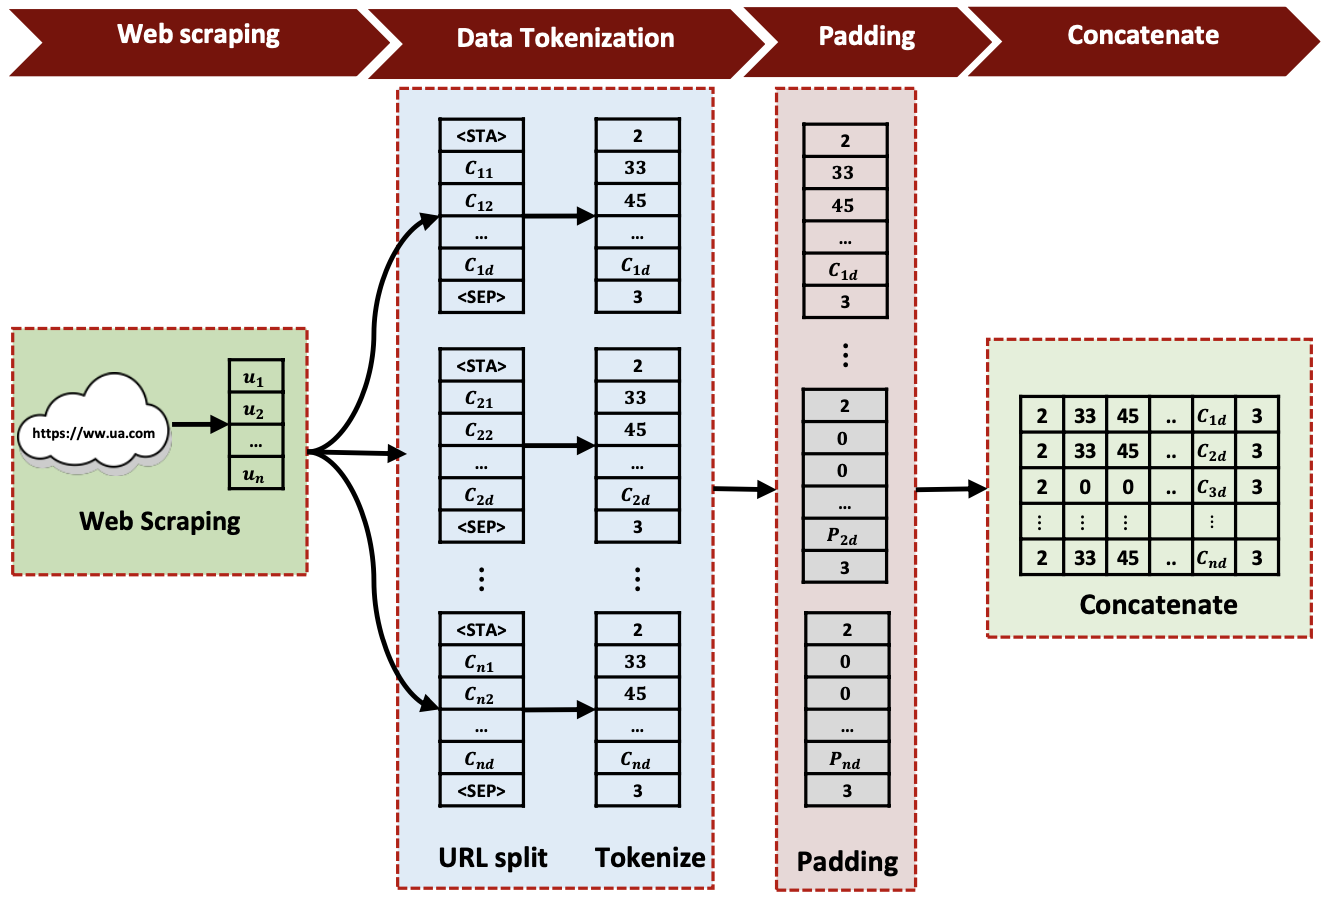
\includegraphics[width=0.8\linewidth]{images/transformer preprocessing.png}
    \caption{URL Preprocessing}
    \label{fig:URL Preprocessing}
\end{figure}

\subsubsection{Model structure}
The URLs constructed in this manner are then concatenated and are ready to be passed to the CNN. After this, a max pooling layer is applied to extract the most important features and significantly reduce the input space. A flatten layer is then used to convert the multi-dimensional array into a one-dimensional array, making it ready to be passed to the encoder.

The encoder is capable of capturing dependencies between the various symbols using the multi-head attention mechanism. Each character is associated with its position through a positional encoder. Then, each vector embedding is multiplied by three randomly initialized weights, called Query (Q), Key (K), and Value (V). The self-attention layer calculates a score for each character relative to the current character using the following formula:
\begin{equation}
Z(Q, K, V) = \text{softmax}\left(\frac{QK^T}{\sqrt{d_k}}\right)V
\end{equation}
Finally, a normalization layer is applied, which takes the self-attention output \(Z\) and the input \(X\) to stabilize the model's training. The encoder's output is passed through a max-pooling layer and then to a fully connected layer for classification.

\subsubsection{Model Parameters and Training}
The model was trained using K-fold cross-validation with \(k = 5\), and the hyperparameters used are shown in the figure below.

\begin{figure}[htp]
    \centering
    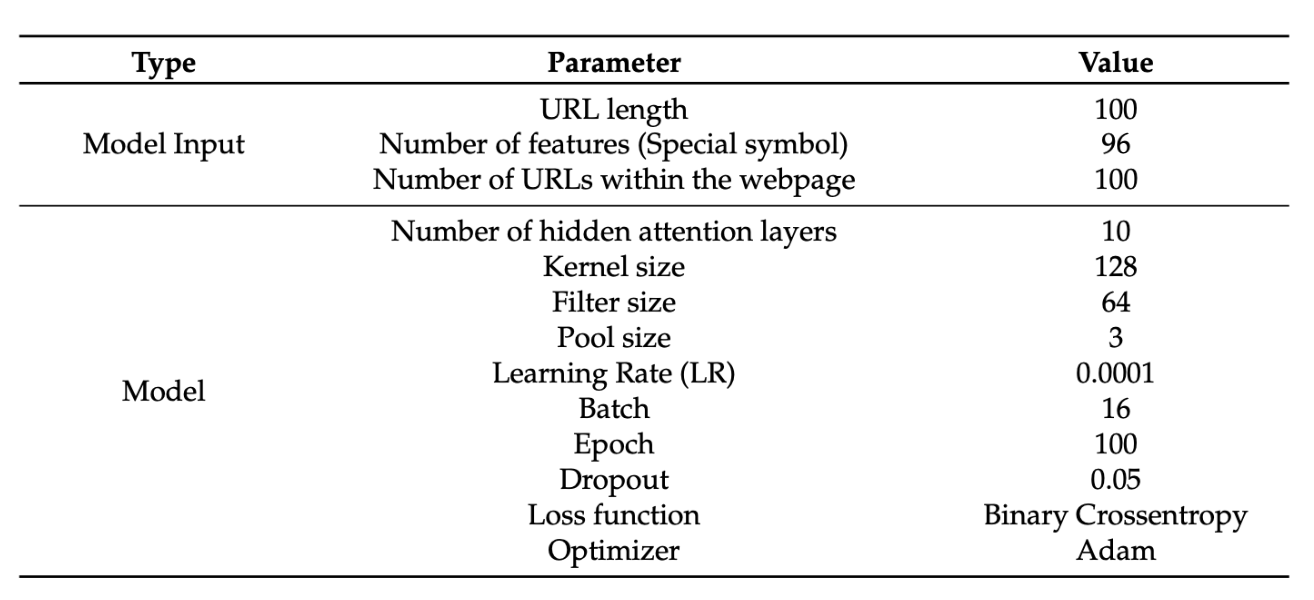
\includegraphics[width=1\linewidth]{images/Transformer parameters.png}
    \caption{CNN+Transformer parameters}
    \label{fig:CNN+Transformer parameters}
\end{figure}

\subsection{Models Evaluations}
 The generated model was compared with SVM, a CNN, and a biLSTM (which consists of two LSTMs—one processes the sequence from the first to the last element, and the other processes the sequence from the last to the first element). Additionally, two state-of-the-art models were considered as baseline models, both URL-based but differing in feature extraction and classification methods. URLNET is based on a CNN and performs feature extraction at three levels: character, word, and character-word. On the other hand, MPURNN is based on a biLSTM and focuses on character-level features.
\begin{figure}[htp]
    \centering
    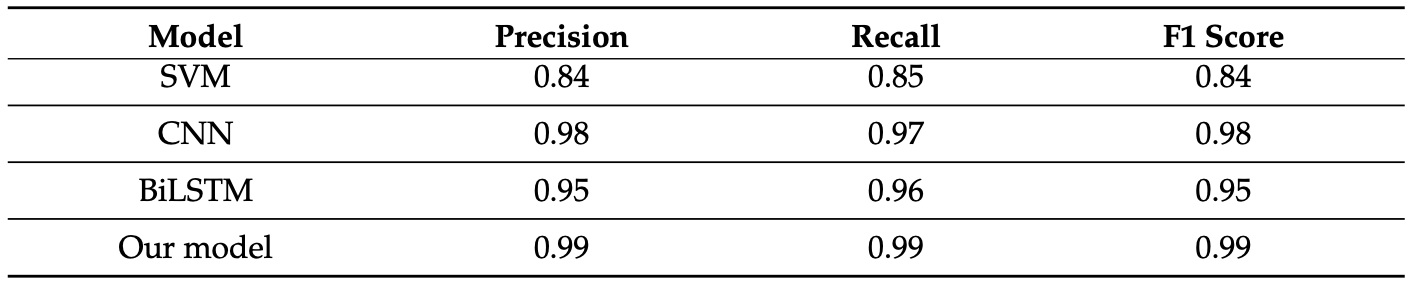
\includegraphics[width=1\linewidth]{images/TransformerComparison1.png}
    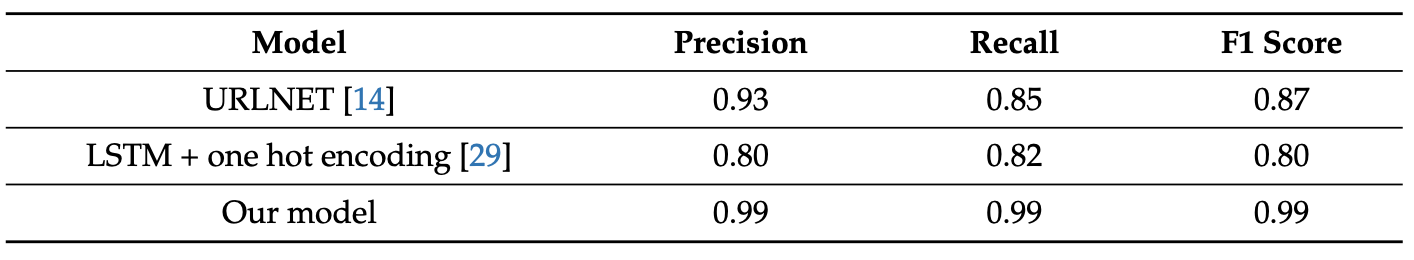
\includegraphics[width=1\linewidth]{images/TransformerComparison2.png}
    \caption{Models Comparison}
    \label{fig:Models Comparison}
\end{figure}
As we can see, in all cases, the model proposed by the authors outperforms the state-of-the-art models, achieving near-perfect performance with 99\% precision, recall, and F1-score.
\chapter{Discussion}
\section{Solutions comparison}

\begin{table}[h]
    \centering
    \begin{tabular}{lcccc}
        \toprule
        \textbf{Model name} & \textbf{Accuracy} & \textbf{Precision} & \textbf{Recall} & \textbf{F1 score} \\ 
        \midrule
        EPDB & 99.36 & 98.87 & 100.00 & 99.43 \\
        PDGAN & 97.58 & 98.02 & 97.27 & 97.64 \\
        PhishingTransformer & 98.90 & 98.80 & 99.00 & 98.80 \\
        \bottomrule
    \end{tabular}
    \caption{Solutions Comparison}
    \label{tab:solutions_comparison}
\end{table}

\textbf{EPDB} achieves the highest performance metrics, but it's important to note that this result is based on a relatively small dataset of 11,055 records. The exceptional results could indicate that the model is well-tuned for the specific dataset but might require further validation on larger, more diverse datasets to ensure its robustness in broader applications.

\textbf{PhishingTransformer} also shows strong performance with a dataset of 100,000 records. This model strikes a good balance between precision and recall, demonstrating its effectiveness on a moderately sized dataset. Its near-perfect metrics suggest that it generalizes well, even with a significantly larger dataset than EPDB's.

\textbf{PDGAN}, despite using a much larger dataset of 2.3 million records, has slightly lower performance metrics. This could suggest that while PDGAN is effective at processing large-scale data and maintaining high precision, it faces challenges in achieving the same level of recall and overall accuracy as the other models. However, its ability to handle such a large dataset indicates its scalability and potential for real-world applications where large volumes of data are common.

\section{Considerations}
Qualitatively, the datasets used by the authors of the three models differ from each other, but they mostly come from the same sources, so they can be assumed to be fairly similar. However, quantitatively, they cannot be considered similar since the \textbf{EPDB} dataset is one-tenth the size of the \textbf{PhishingTransformer} dataset, which is 20 times smaller than the \textbf{PDGAN} dataset. Therefore, it is difficult to determine the absolute best model.

Regarding the \textbf{EPDB} model, we have information on its performance in terms of execution speed 4 seconds for the Random Forest model. The other deep learning solutions are undoubtedly more complex and require more time both during training and inference.

The authors of \textbf{EPDB} and \textbf{PhishingTransformer} use the k-fold cross-validation technique to obtain more reliable and stable statistical estimates of model performance. However, the authors of \textbf{PhishingTransformer} use this technique to allow the model to learn from the validation set as well, as explained in their paper in section 4.5: \textit{"Therefore, it ensures that every data point contributes to training and validation, maximizing the utilization of our dataset."} This approach, however, does not utilize k-fold cross-validation but rather trains the same model five times on the entire training dataset (80\% of the total). This is also evident from the graph provided by the authors, where the model's performance, instead of varying slightly, increases sharply after the first fold and reaches perfection by the fifth fold, likely resulting in overfitting.

\begin{figure}[htp]
    \centering
    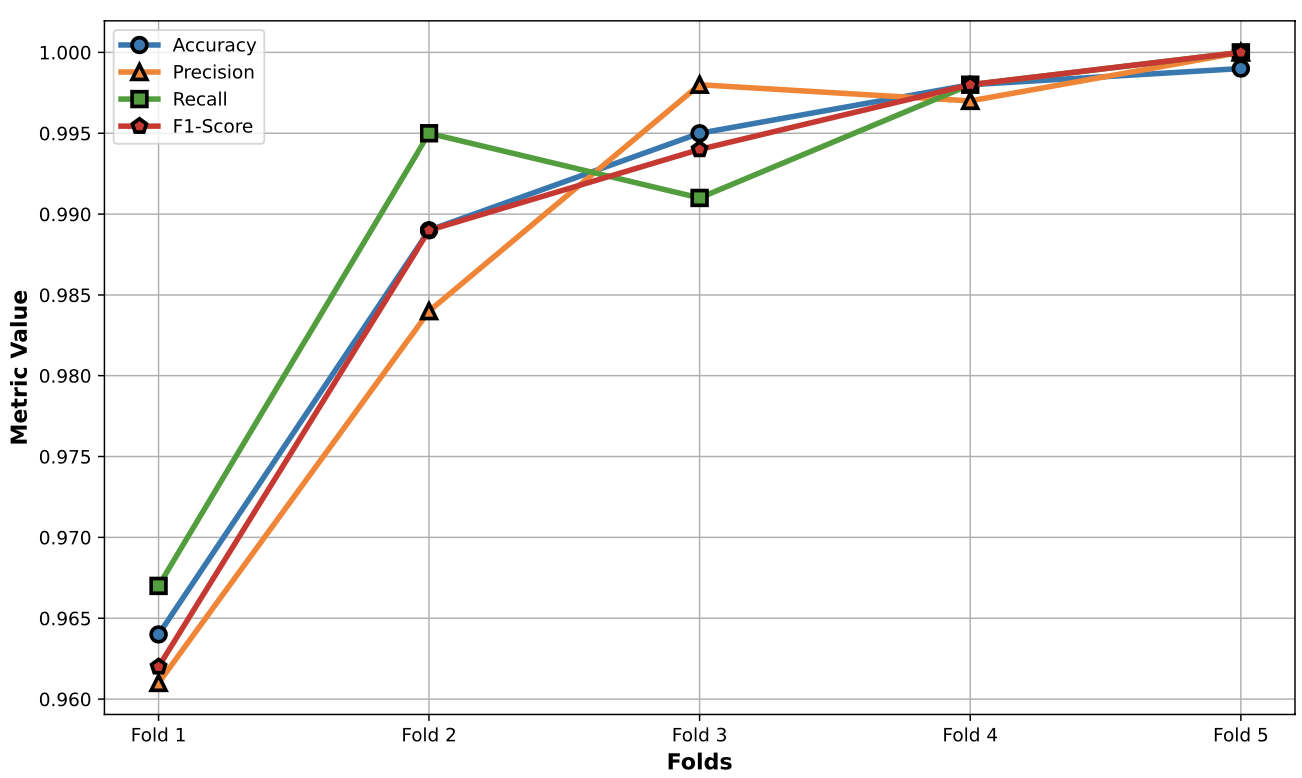
\includegraphics[width=0.8\linewidth]{images/K-fold errror.png}
    \caption{Five-fold cross validation}
    \label{fig:Five-fold cross validation}
\end{figure}
The authors of \textbf{DPGAN} created a model that not only can distinguish between a safe and an unsafe website but also is capable of generating new URLs. They use the generator to create 50,000 synthetic URLs and add them to the dataset to improve the model's performance. This technique is not universally accepted among researchers because, while it offers the advantage of data augmentation and helps address data scarcity, it also has the drawback of potentially leading to overfitting on synthetic data. The discriminator might become overly reliant on synthetic data, reducing its effectiveness on real data. However, in this case, considering that the synthetic data accounts for only 1/40th of the total dataset, the model's improvement can be accepted without significant concern for overfitting on synthetic data.

Regarding hyperparameter optimization, \textbf{EPDB} uses GridSearchCV, ensuring that the best possible results are obtained. Similarly, \textbf{PDGAN} involved varying hyperparameters to choose the optimal solution. On the other hand, for \textbf{PhishingTransformer}, assumptions were made regarding the length of URLs and the number of embedded URLs, while the other CNN hyperparameters were left at their default settings.

However, \textbf{PhishingTransformer} introduces an interesting hybrid-based solution compared to the other two URL-based solutions, which helps prevent phishing attacks through "embedding malicious code in legitimate content."

\section{Conclusion and future improvements}
The authors of PDGAN and PhishingTransformer propose an innovative AI model, which uses a CNN to extract URL features and an LSTM or Encoder to understand the relationships between URL characters. In contrast, the authors of EPDB present a complete system, specifically a secure browser. With some modifications, it might be possible to replace or integrate the ML prediction model with one of the deep learning techniques proposed by the other authors.

It could also be interesting to explore continuous or federated learning techniques to keep the models continuously updated without the need to retrain the entire model, which, especially in the case of Deep Learning  techniques, becomes particularly time-consuming.

As potential improvements, increasing the dataset for EPDB is essential, as it is too small, and similarly for PhishingTransformer, which, although ten times larger than EPDB’s, still remains a deep learning technique that requires much more data to effectively learn the network weights. Additionally, a model could be developed that incorporates predictions from all three models and makes a decision based on a weighted average.


\end{document}